\chapter{Dokumentacja użytkownika}\label{chap:dokumentacja-uzytkownika}
W niniejszym rozdziale opisano sposób korzystania z aplikacji. Jak widać na diagramie przypadków użycia z rysunku \ref{image:przypadki-uzycia}, aplikacja zawiera dwa główne scenariusze wykonania.
\begin{figure}[h]\label{fig:xamarin_model}
\begin{center}
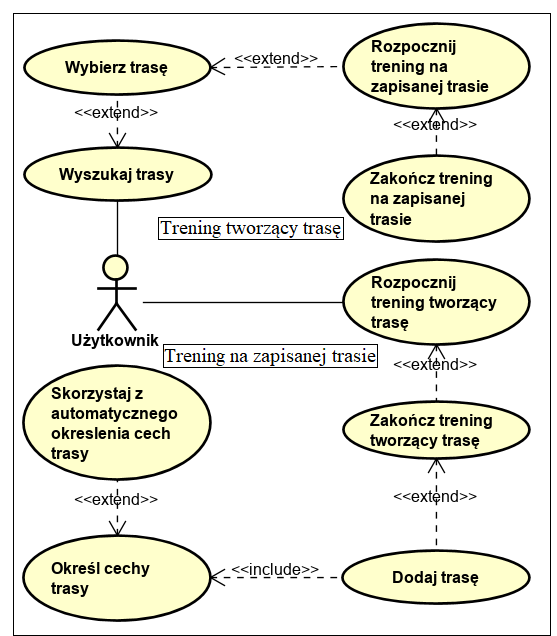
\includegraphics{img/przypadki-uzycia.png}
\caption{Diagram przypadków użycia [Opracowanie własne]}\label{image:przypadki-uzycia}
\end{center}
\end{figure}

\section{Trening tworzący trasę}
Po uruchomieniu aplikacji użytkownikowi ukazuje się ekran główny. Wciśnięcie przycisku „START” powoduje rozpoczęcie treningu i uruchomienie stopera. Wraz z przemieszczaniem się, na mapie rysowana jest linia reprezentująca pokonany dystans. Sytuację tę pokazano na rysunku \ref{image:tworzenie-screen}.
\begin{figure}
\centering
\begin{minipage}{.5\textwidth}
  \centering
  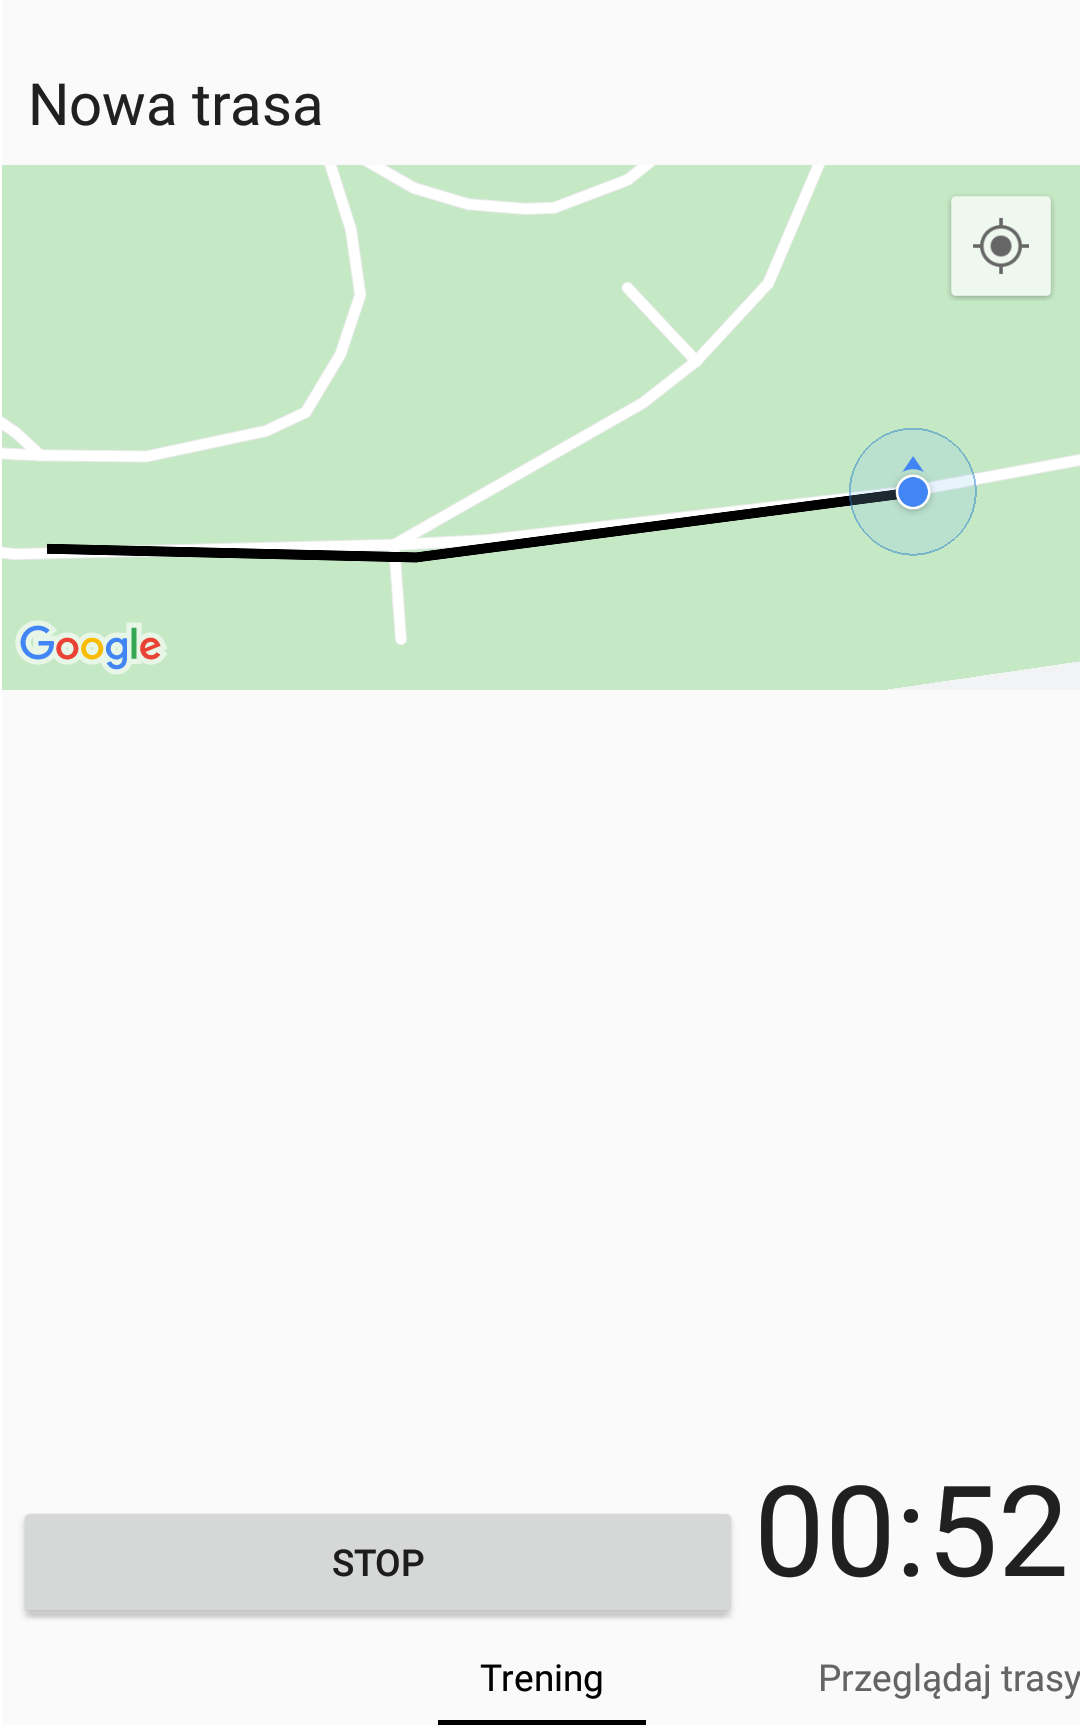
\includegraphics[width=.8\linewidth,frame]{img/tworzenie}
  \captionof{figure}{Widok podczas tworzenia trasy [Opracowanie własne]}
  \label{image:tworzenie-screen}
\end{minipage}%
\begin{minipage}{.5\textwidth}
  \centering
  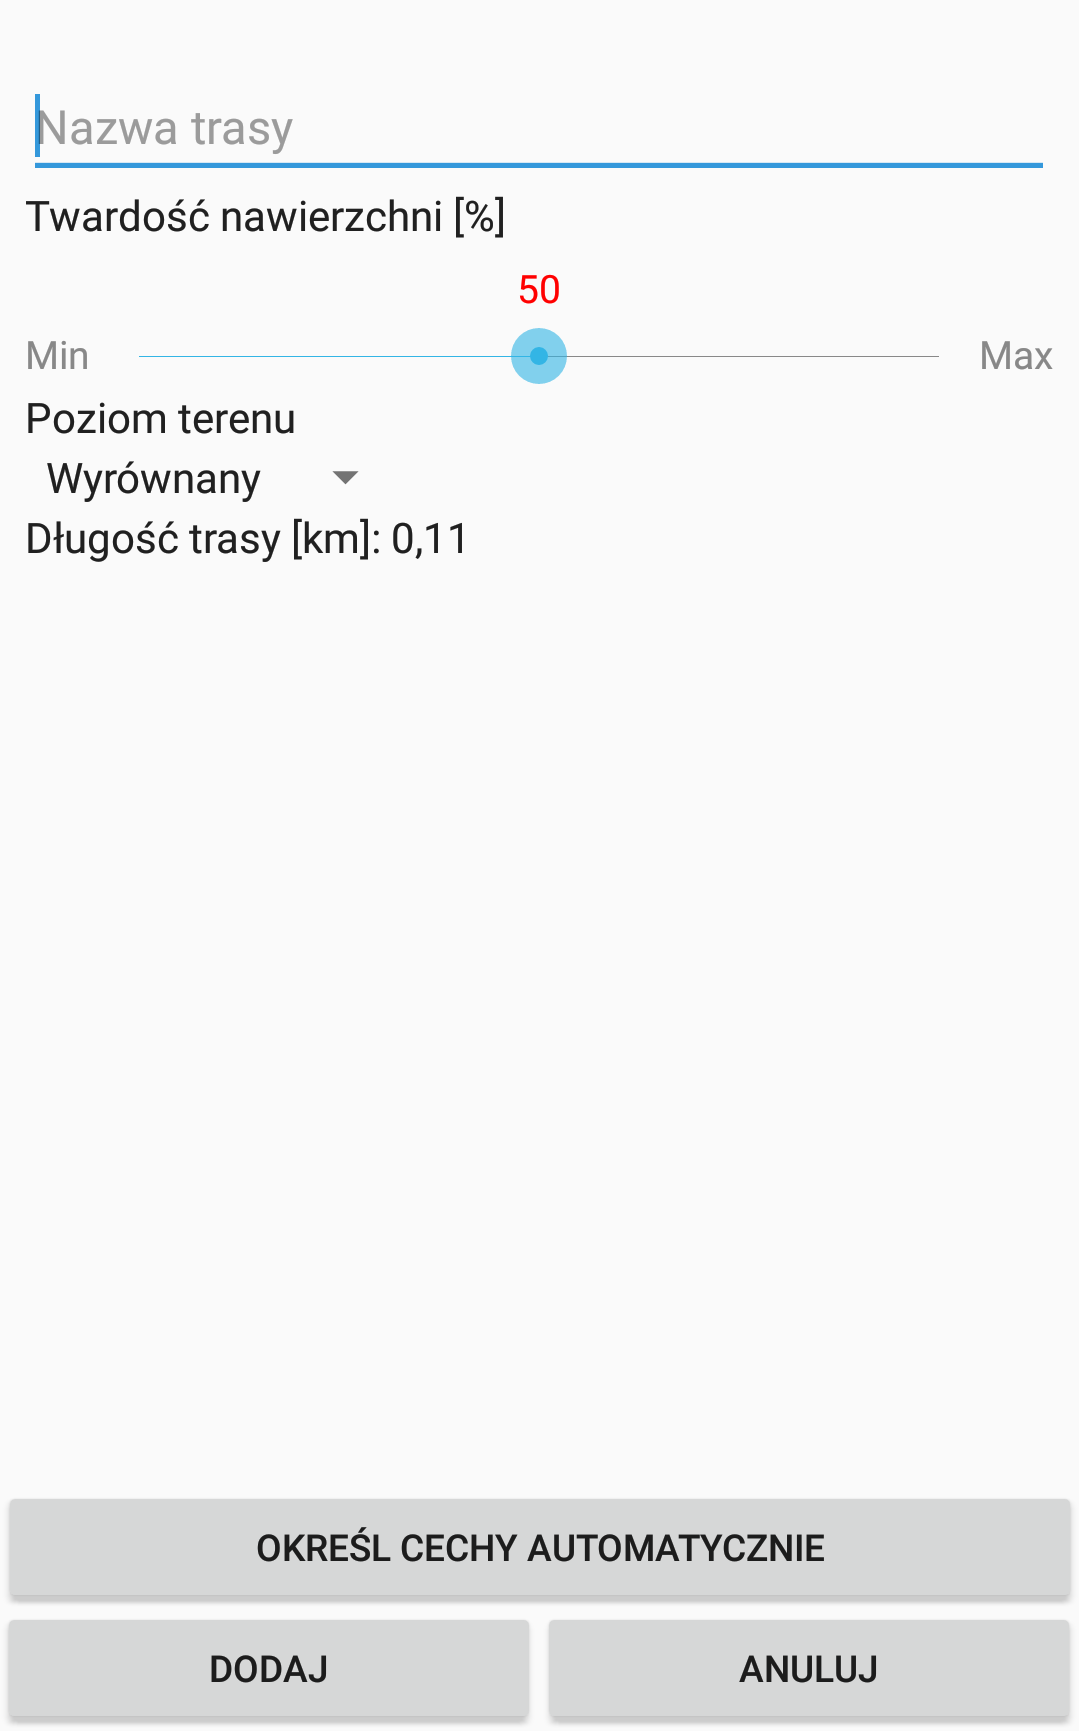
\includegraphics[width=.8\linewidth,frame]{img/cechy}
  \captionof{figure}{Widok podczas określania cech trasy [Opracowanie własne]}
  \label{image:cechy-screen}
\end{minipage}
\end{figure}

Po wciśnięciu przycisku „STOP” trening zostaje przerwany, a oczom użytkownika ukazuje się widok pokazany na rysunku \ref{image:cechy-screen}. W tym momencie zadaniem użytkownika jest wpisanie nazwy trasy oraz określenie jej cech. Wciśnięcie przycisku „OKREŚL CECHY AUTOMATYCZNIE” spowoduje oszacowanie cech trasy i odpowiednie zaktualizowanie suwaka określającego twardość trasy oraz wybranego poziomu terenu. Wciśnięcie przycisku „DODAJ” doprowadzi do dodania trasy do systemu, natomiast skorzystanie z przycisku „ANULUJ” spowoduje odrzucenie wykonanego treningu.

\section{Trening na zapisanej trasie}
Po wciśnięciu przycisku  „Przeglądaj trasy” umiejscowionego na dole ekranu, użytkownik zostaje przeniesiony do widoku wyszukiwania tras. Jego układ został pokazany na rysunku \ref{image:wyszukiwanie}. Biegacz ma możliwość określenia kryteriów wyszukiwania. Po wciśnięciu przycisku „SZUKAJ” oczom użytkownika ukazuje się lista tras. Przełączanie pozycji listy odbywa się poprzez przewijanie listy w górę oraz w dół ekranu. Dla każdej trasy oprócz jej cech oraz nazwy, pokazana jest także mapa, która obrazuje jej umiejscowienie.
\begin{figure}[h]\label{fig:xamarin_model}
\begin{center}
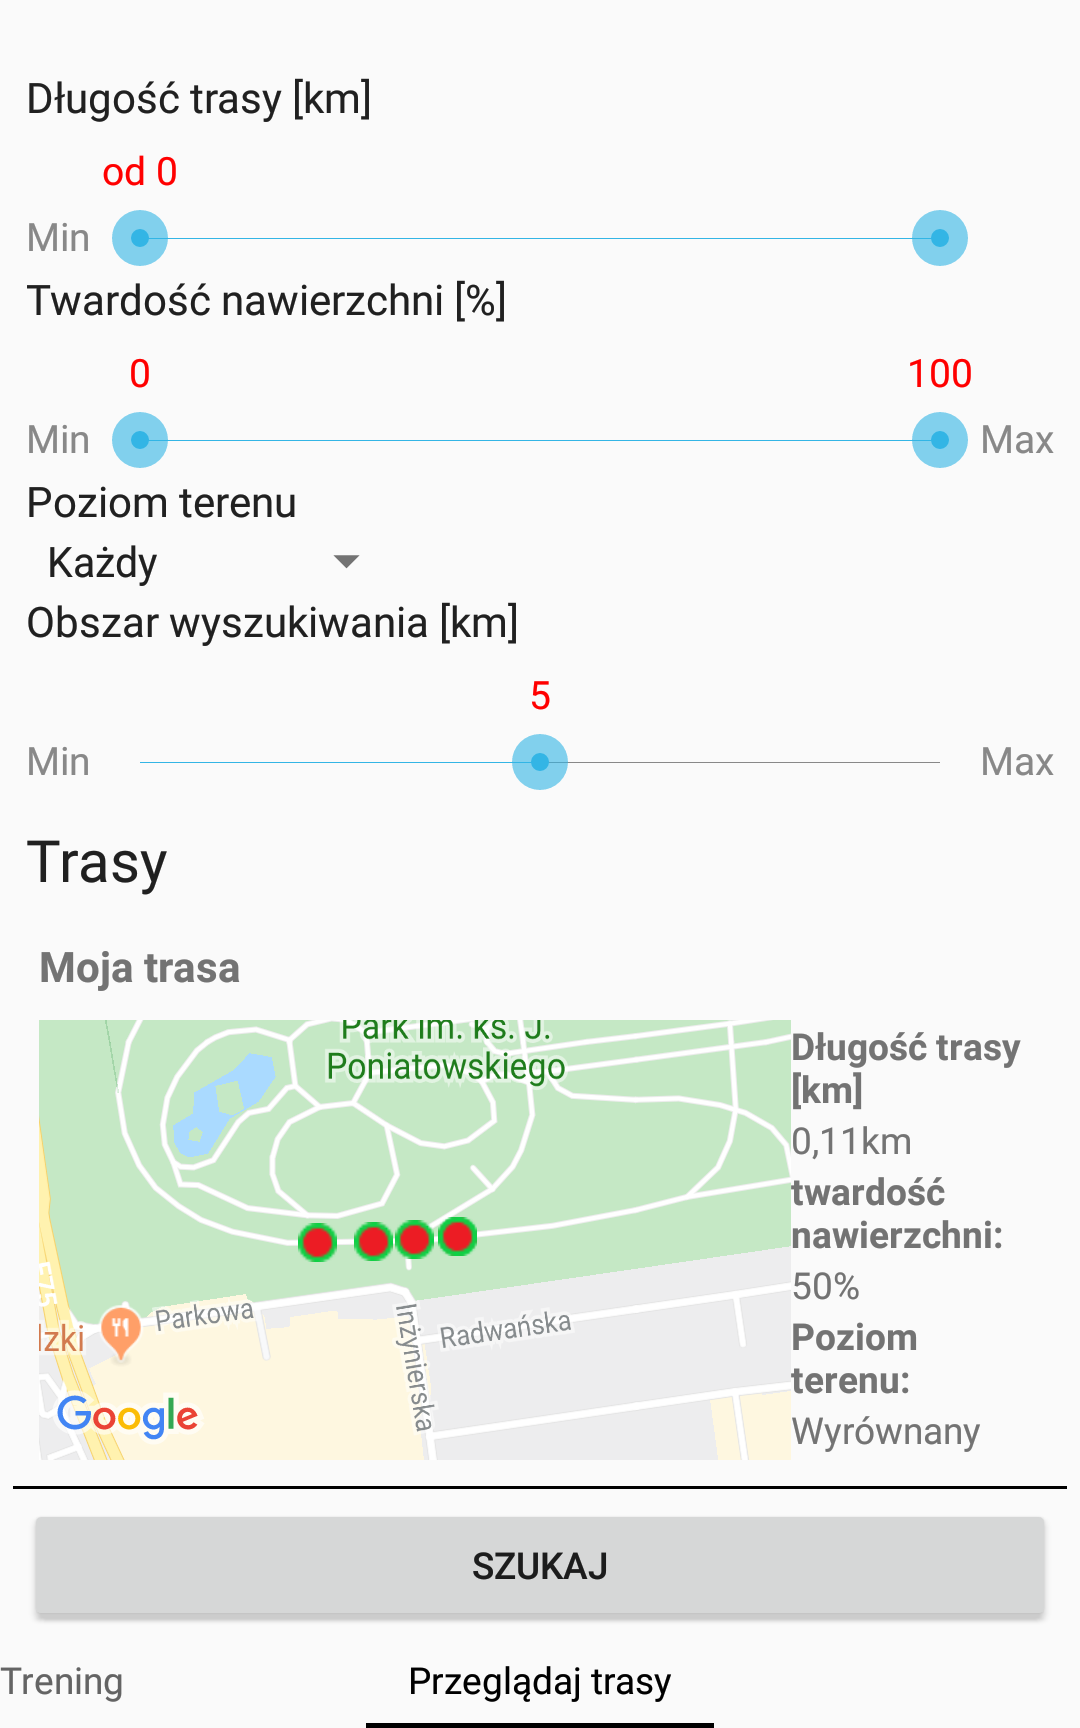
\includegraphics[width=.5\linewidth,frame]{img/wyszukiwanie.png}
\caption{Widok wyszukiwania tras [Opracowanie własne]}\label{image:wyszukiwanie}
\end{center}
\end{figure}

Wybranie trasy odbywa się poprzez wciśnięcie odpowiedniej pozycji na pokazanej liście. W wyniku tego działania użytkownik zostaje przeniesiony do widoku, który pokazano na rysunku \ref{image:rywalizacjaw1}. Na mapie pokazane są punkty kontrolne, przypisane do trasy. Dodatkowo wyświetlony jest ranking, na którym umieszczone są czasy wszystkich użytkowników, którzy ukończyli wybraną trasę. Kolorem zielonym oznaczona jest próba użytkownika, który korzysta z aplikacji. W momencie gdy ilość biegaczy, która zapisana jest w rankingu nie mieści się na ekranie, możliwe jest przesunięcie listy w górę lub w dół i zobaczenie brakujących pozycji.

Wciśnięcie przycisku „START” powoduje rozpoczęcie wirtualnej rywalizacji. Na koniec rankingu dodawana jest wyróżniona kolorem niebieskim pozycja o nazwie „Obecna próba”. Reprezentuje ona wynik osiągany w ramach bieżącego treningu. Zadaniem użytkownika jest przebiegnięcie w odległości nie większej niż 15 metrów od każdego z punktów kontrolnych. Za każdym razem gdy punkt kontrolny zostanie osiągnięty, pozycje użytkowników w rankingu są aktualizowane. Oprócz tego pokazywany jest czas uzyskany na tym punkcie kontrolnym.  Dodatkowo na urządzeniu odtwarzane są komunikaty głosowe informujące o aktualnie zajmowanej pozycji lub (w przypadku zmiany pozycji użytkownika w rankingu) także o liczbie zyskanych lub utraconych miejsc. Przykład trwającego procesu wirtualnej rywalizacji został pokazany na rysunku \ref{image:rywalizacjaw2}.

Wraz z postępem treningu osiągnięte punkty kontrolne są usuwane, a mapa przesuwa się tak, aby następny w kolejności punkt kontrolny znajdował się na jej środku. W razie wątpliwości pomaga to zorientować się, jaki kierunek należy obrać. Osiągnięcie ostatniego punktu kontrolnego powoduje automatyczne zakończenie treningu. W przypadku osiągnięcia wyniku lepszego niż w ramach poprzedniej próby, nowy czas zostanie zapisany w systemie.
\begin{figure}
\centering
\begin{minipage}{.5\textwidth}
  \centering
  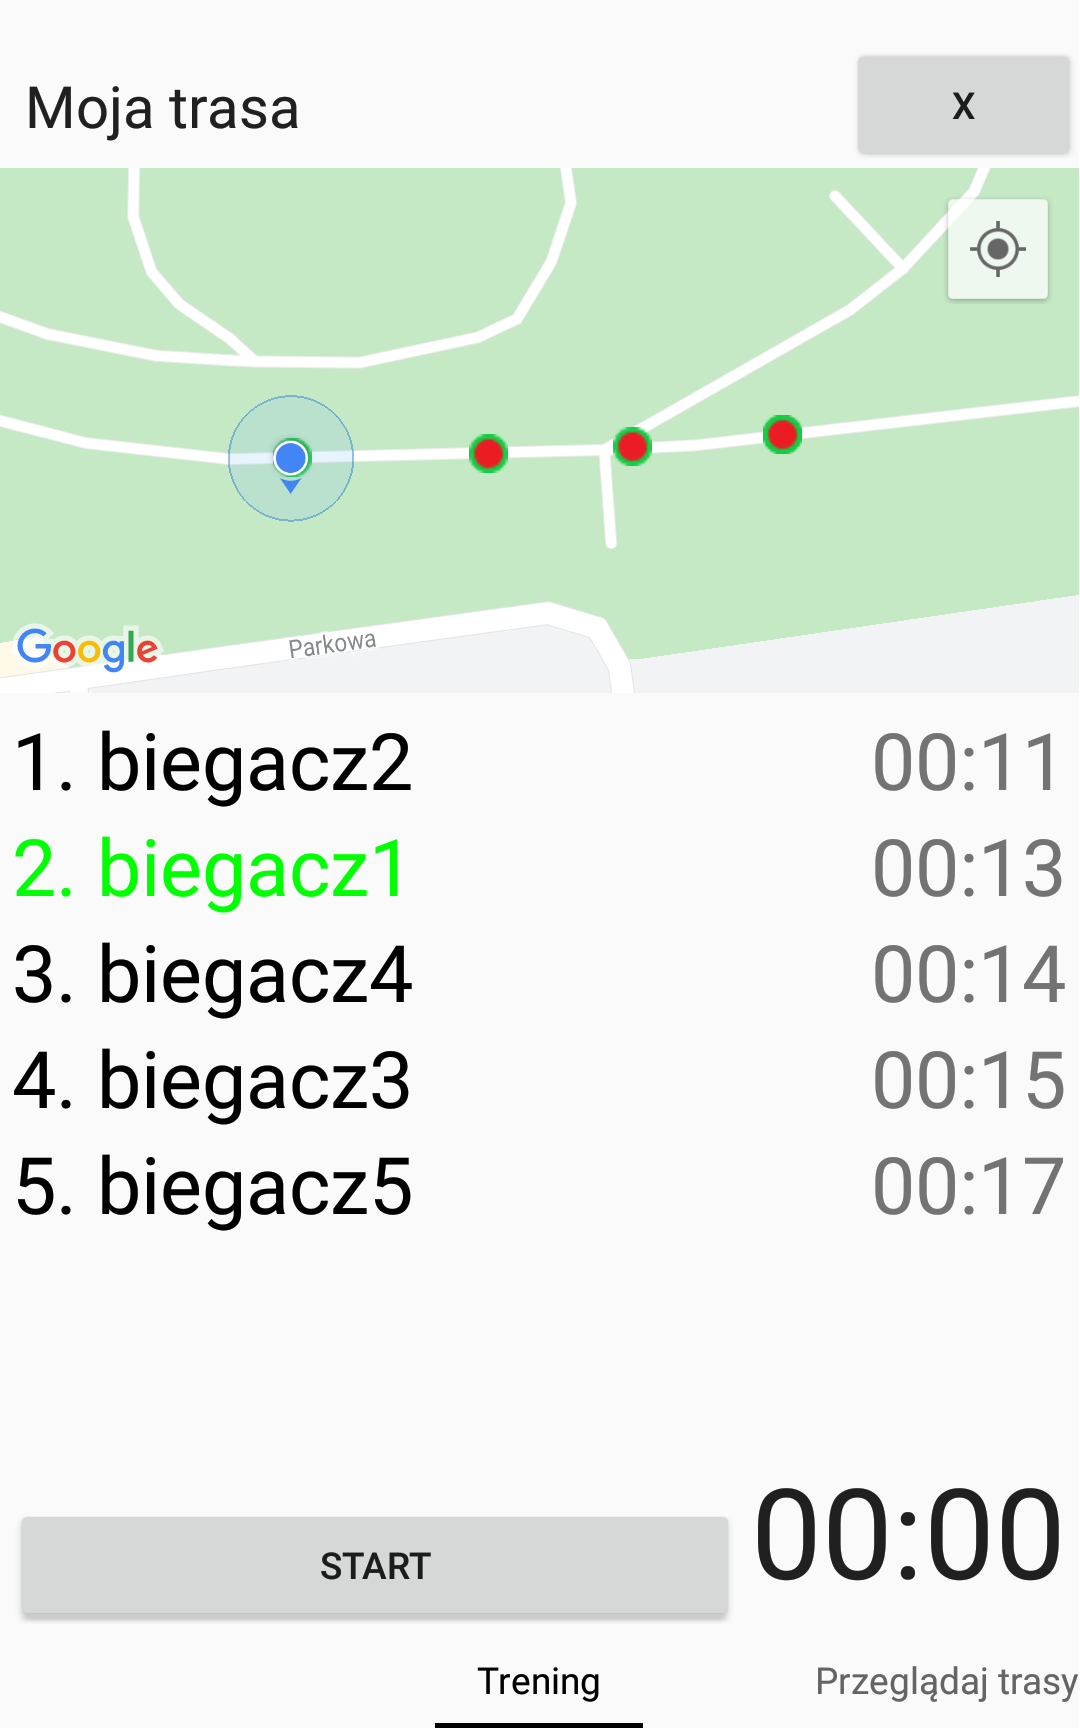
\includegraphics[width=.8\linewidth,frame]{img/rywalizacjaw1}
  \captionof{figure}{Widok przed rozpoczęciem wirtualnej rywalizacji [Opracowanie własne]}
  \label{image:rywalizacjaw1}
\end{minipage}%
\begin{minipage}{.5\textwidth}
  \centering
  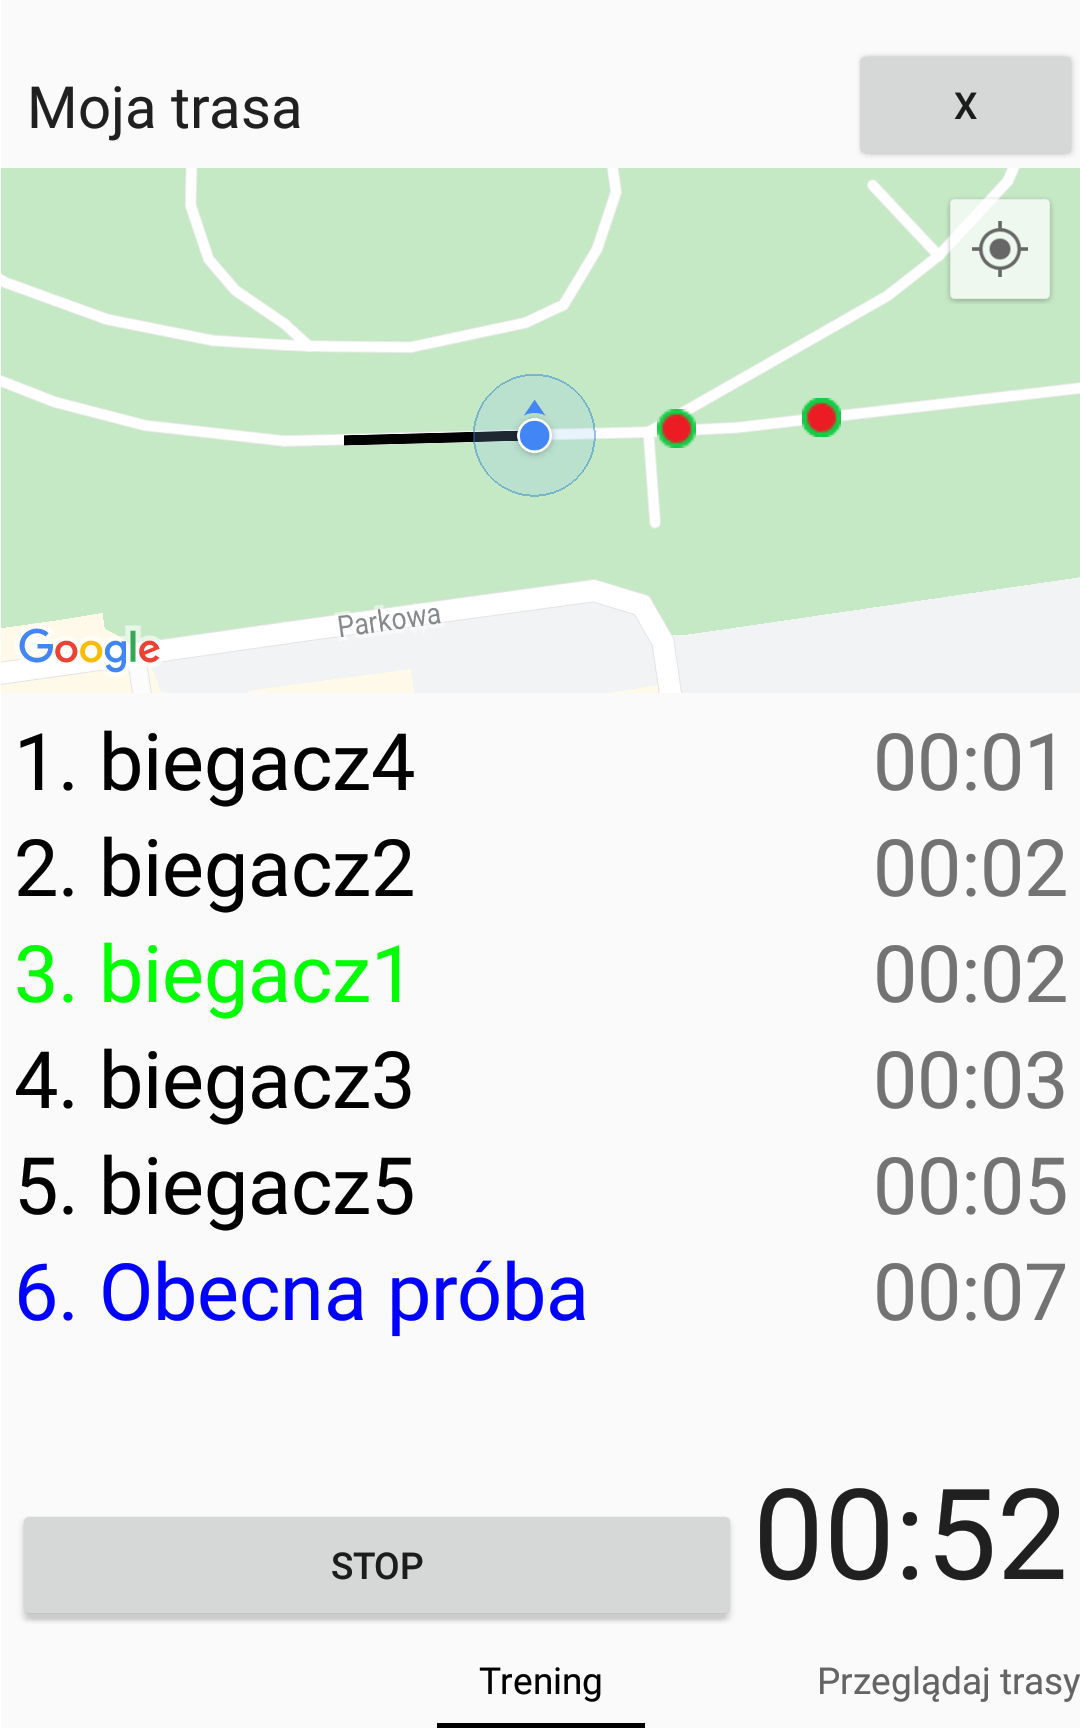
\includegraphics[width=.8\linewidth,frame]{img/rywalizacjaw2}
  \captionof{figure}{Widok podczas wirtualnej rywalizacji [Opracowanie własne]}
  \label{image:rywalizacjaw2}
\end{minipage}
\end{figure}